\label{sec-methodology}

\subsection{Base, canal e protocolo de rótulos}

A MIT-BIH Arrhythmia Database reúne registros ambulatoriais de cerca de
30 minutos, amostrados a 360 Hz em dois canais
\citep{moody2001mitdb,physionetmitdb}. O pipeline lê os arquivos locais com
WFDB, prioriza o canal MLII quando disponível e usa as anotações \texttt{atr}
como referência temporal dos batimentos. Após a exclusão dos registros
paced-heavy \texttt{102}, \texttt{104}, \texttt{107} e \texttt{217}, o
protocolo mantém 44 registros.

O rótulo binário é usado apenas na avaliação. Batimentos \texttt{N} formam a
classe normal, enquanto os demais símbolos válidos de batimento formam a classe
anômala. Símbolos técnicos, mudanças de ritmo e batimentos paced ficam fora da
amostra analisável. Essa escolha preserva o foco em anomalias de batimento
não-paced e evita transformar o benchmark em um detector de marcapasso.

\subsection{Segmentação e filtragem do sinal de entrada}

Cada linha experimental corresponde a uma janela de 0,25 s antes e 0,45 s
depois da anotação. Janelas que encostam nas bordas do registro são descartadas
para preservar duração constante. O sinal é filtrado no registro completo antes
da segmentação, pois aplicar \texttt{filtfilt} diretamente em janelas curtas
introduziria artefatos de borda.

A cadeia adotada remove primeiro a média do registro e, em seguida, aplica dois
filtros FIR lineares com janela de Hamming e fase zero por forward-backward. O
primeiro é um passa-alta em 0,5 Hz com largura de transição de 1 Hz e
1189 coeficientes. O segundo é um passa-baixa em 40 Hz com largura de
transição de 8 Hz e 149 coeficientes. A escolha combina preservação da
morfologia útil do ECG com atenuação de deriva de linha de base, ruído muscular
e componentes de alta frequência \citep{thakor1984qrs,elgendi2017efficient,butt2020signalpiloted}.
Como o R-peak serve de âncora para a segmentação e para as janelas fisiológicas
de P, QRS e T, a filtragem em fase zero evita deslocamentos temporais que
prejudicariam a interpretação local do batimento.

Nenhuma feature é extraída do sinal bruto. Todos os descritores do manuscrito
partem desse sinal filtrado comum, o que reduz a influência de ruído residual
na comparação entre os modelos e mantém a base fisiológica da representação.

\begin{figure}[!htbp]
  \centering
  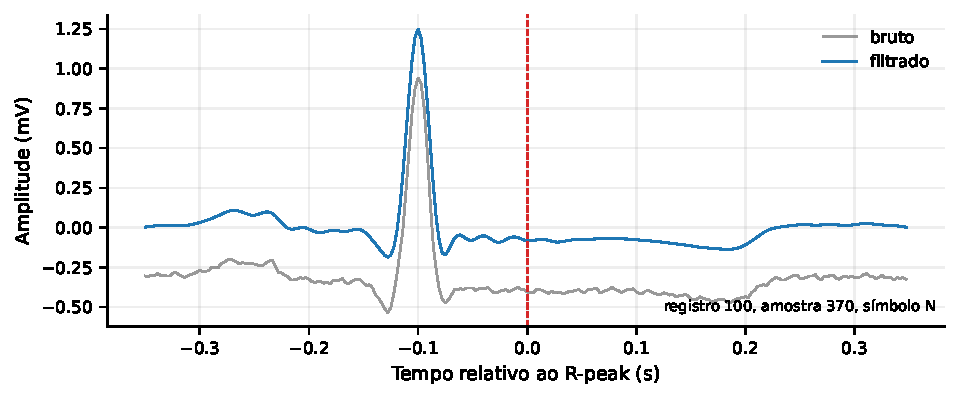
\includegraphics[width=0.95\linewidth]{figures/fig_raw_vs_filtered_beat.pdf}
  \caption{Batimento normal segmentado no mesmo R-peak antes e depois da cadeia FIR.}
  \label{fig-raw-filtered}
\end{figure}

\subsection{Split inter-paciente e tamanho do dataset}

Os registros do grupo DS1 formam o conjunto de treino e os registros DS2 formam
o teste final. Nenhum paciente aparece nos dois lados. Depois da filtragem, da
segmentação e das exclusões, o protocolo produziu 100.694 batimentos válidos.
Desse total, 74.516 pertencem à classe normal e 26.178 à classe anômala. O
treino contém 51.002 batimentos, com 38.088 normais e 12.914 anômalos. O teste
contém 49.692 batimentos, com 36.428 normais e 13.264 anômalos.
